\subsection*{Ingresos y egresos}
\addcontentsline{toc}{subsection}{Ingresos y egresos}

\subsubsection*{Ingresos}
\addcontentsline{toc}{subsubsection}{Ingresos}

Para desarrollar el plan de negocios propuesto, se definieron dos planes para acceder a las funcionalidades de venta de la plataforma. En primer lugar, se encuentra el plan gratuito, el cual se presenta no solo como una opción de prueba para uso general, sino que también está dirigido a usuarios que deseen explorar la plataforma con un número limitado de accesos a contenidos interactivos y la muestra de publicidad dentro de la plataforma.

Por otra parte, el plan de suscripción habilita funcionalidades adicionales, tales como el acceso a una mayor cantidad de contenidos y más alternativas de inversión sin la necesidad de recurrir en anuncios.

En la tabla \ref{TablaIngresos} se presenta de manera más detallada el análisis de los ingresos mensuales y anuales proyectados para la compañía.

\begin{table}[H]
	\centering
	\caption[{Tabla de ingresos}]{\centering Tabla de ingresos. \textit{Fuente:} Autores.}
	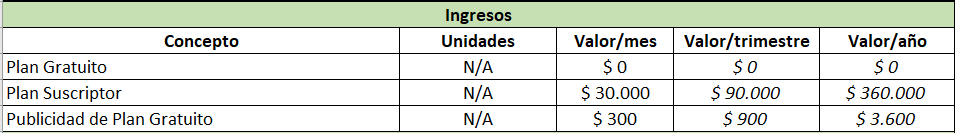
\includegraphics[width=14cm]{Imagenes/TablaIngresos.png}
	\label{TablaIngresos}
\end{table}

\subsubsection*{Egresos}
\addcontentsline{toc}{subsubsection}{Egresos}

Durante el primer año se deben tener en cuenta las siguientes consideraciones. En primer lugar, el proyecto será liderado por dos personas, por lo que inicialmente se contará con un equipo de trabajo reducido. Los pagos correspondientes al personal incluirán las prestaciones sociales, aportes parafiscales, cesantías, primas y demás obligaciones laborales establecidas por la normativa colombiana vigente.

Adicionalmente, se contemplan los costos asociados a la infraestructura necesaria para el desarrollo del trabajo en modalidad virtual. Estos aspectos se presentan con mayor detalle en la tabla \ref{TablaEgresos}.

\begin{table}[H]
	\centering
	\caption[{Tabla de egresos}]{\centering Tabla de egresos. \textit{Fuente:} Autores.}
	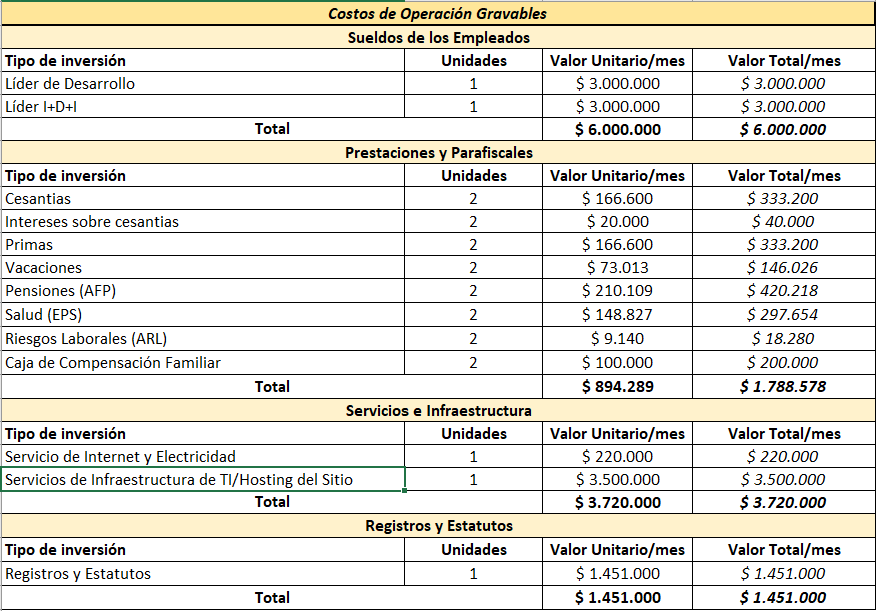
\includegraphics[width=15cm]{Imagenes/TablaEgresos.png}
	\label{TablaEgresos}
\end{table}